\chapter{Test}
\label{chap:test}

\section{Test ``Analisi assistita''}

\subsection{Sito web: SudokuWorld}

\subsubsection{Total Validator}
\begin{figure}[H]
    \centering
    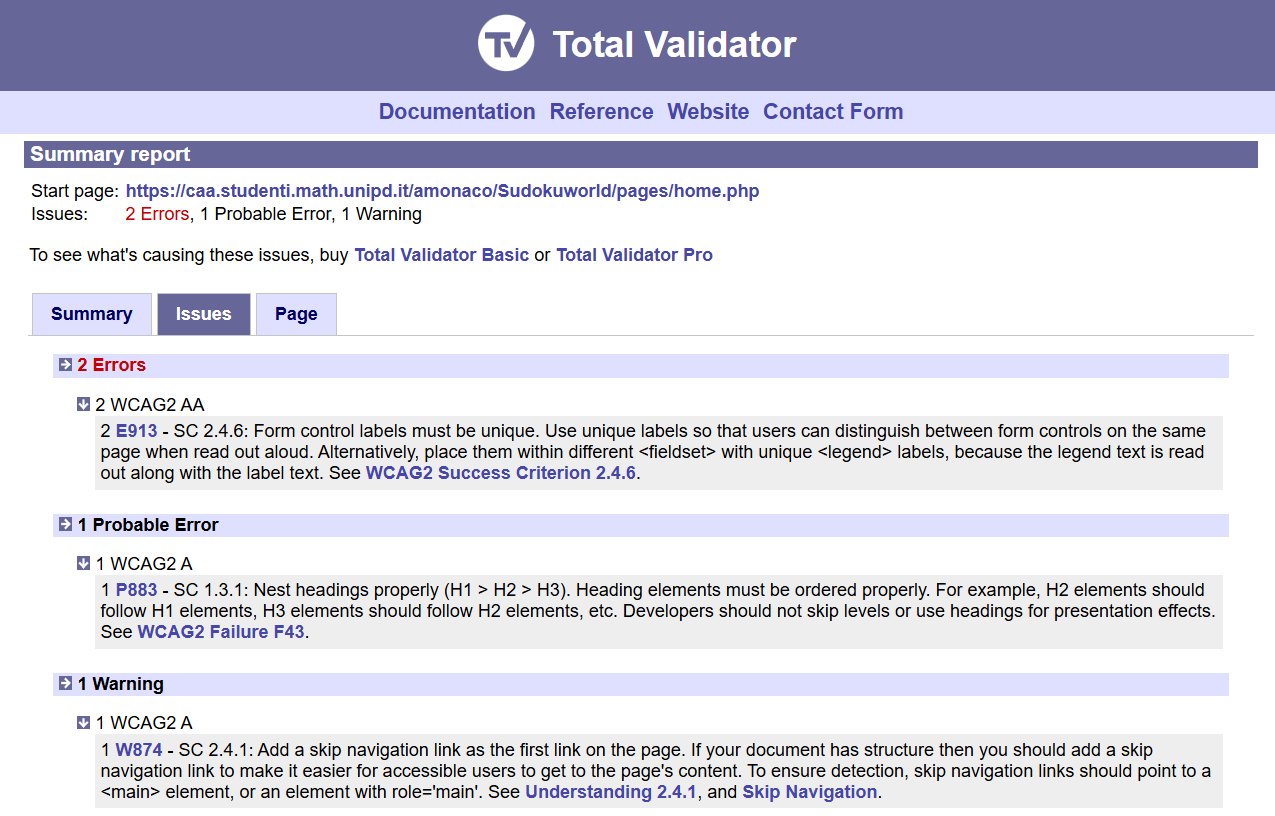
\includegraphics[width=0.7\linewidth, alt={Screenshot dell'analisi di Total Validator sul sito web SudokuWorld}]{img/TV_sudoku.png}
    \caption{Analisi di Total Validator sul sito web SudokuWorld}\label{fig:TV_sudoku}
\end{figure}

\noindent Come visibile nella figura \ref{fig:TV_sudoku} è possibile vedere che lo strumento TV trova ben 15 errori di accessibilità.\\
Gli errori principali sono: 
\begin{itemize}
    \item E913 - SC 2.4.6: Le etichette dei controlli dei form devono essere univoche. Utilizzare etichette univoche consente agli utenti di distinguere i vari controlli presenti sulla stessa pagina quando vengono letti da uno screen reader. In alternativa, è possibile inserirli all’interno di diversi <fieldset> con <legend> univoci, poiché il testo del <legend> viene letto insieme all’etichetta del controllo. Vedi WCAG2 Success Criterion 2.4.6.
    \item E31 - Sono stati rilevati errori ortografici. Le parole non presenti nel dizionario vengono evidenziate e accompagnate da un elenco di possibili sostituzioni (in parentesi).
    \item P883 - SC 1.3.1: Nidificare correttamente le intestazioni (H1 > H2 > H3). Gli elementi di intestazione devono essere ordinati in modo gerarchico. Ad esempio, un elemento H2 dovrebbe seguire un H1, un H3 dovrebbe seguire un H2, e così via. Gli sviluppatori non devono saltare livelli né utilizzare le intestazioni solo per scopi di presentazione. Vedi WCAG2 Failure F43.
\end{itemize}

\subsubsection{SviluppAbile}
\noindent Di seguito vengono riportati i test effettuati con l'estensione \textit{SviluppAbile}.


\subsubsection{Resoconto finale}






\section{Test ``Modalità guidata''}